\documentclass[12pt, letterpaper]{article}
\usepackage[english]{babel}
\usepackage{graphicx}
\usepackage{float}
\usepackage{hyperref}

\title{DAT510 - Assignment 2}
\author{Fr\o ydis J\o rgensen}

\begin{document}
\begin{titlepage}
\maketitle
\end{titlepage}

\begin{abstract}
A one-paragraph summary of the entire assignment - your choices of cryptographic primitives
and their parameters, procedure, test results, and analysis.
\end{abstract}

\section*{Introduction}
A description of the scientific background for your project, including previous work that your
project builds on. (Remember to cite your sources!) The final sentence (analogous to the thesis
statement in a term paper) is the objective of your experiment.

\section*{Design and Implementation}
In this section I am going to go in details on how I implemented each step of the project and explain how it works.

\subsection*{Part 1}
The first part of this assignment required making a secure communication scenario by following 8 steps.
The first step is to decide on some global parameters for a Diffie-Hellman-like key exchange. So Alice and Bob agree on a cyclic group of order p which had to be a prime as 2q +1. This is a so called safe prime and we get it if we take a Sophie Germain prime as q, and we get a new prime. So in this case I used the Sophie Germain prime 359. 2*359 + 1 = 719. So the shared prime number between Alice and Bob is 719. We can therefore say that the cyclic group is Z*719, which means that after the operations done by Diffie-Hellmann key exchange we will end up with a number between g = 2, which was predefined as the generator, and p = 719. Figure \ref{fig:step1} shows the start at my main function where the generator g and the shared prime is defined.

\begin{figure}[H]
  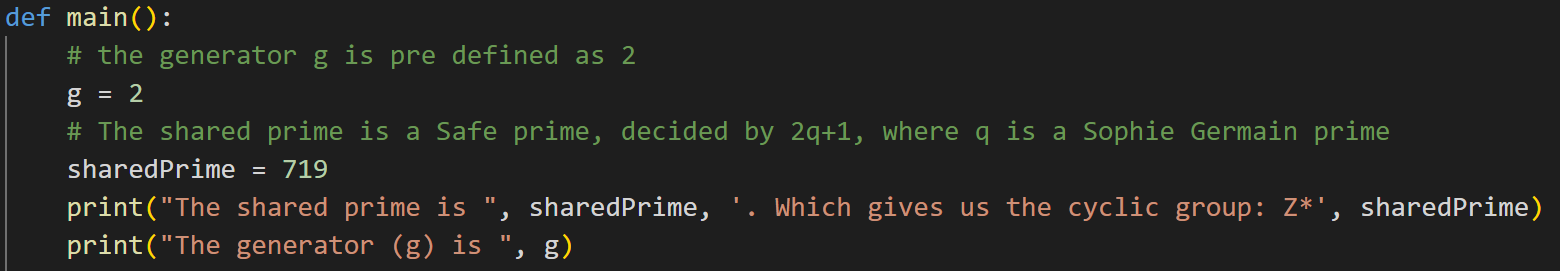
\includegraphics[width=\linewidth]{code_snippets/step1.PNG}
  \caption{Start of my main function, defined g and the shared prime}
  \label{fig:step1}
\end{figure}

The second step is to follow the Diffie-Hellman's key exchange scheme and create Alice and Bobs key pair. For their private key I just chose a random number, so Alice's private key is 217 and Bob's private key is 131. The only requirements for the private keys is that they are smaller than their shared prime and a positive natural number. To create the public key from the private key I created a method, which is shown in Figure \ref{fig:step2_func}. To create the public key, the function does this operation: $$g^{privateKey}\ mod\ sharedPrime$$

\begin{figure}[H]
  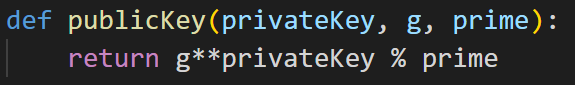
\includegraphics[width=300px]{code_snippets/step2_func.PNG}
  \caption{The function to create the public key}
  \label{fig:step2_func}
\end{figure}

Figure \ref{fig:step2} shows how the private and public key are defined for Alice and Bob.

\begin{figure}[H]
  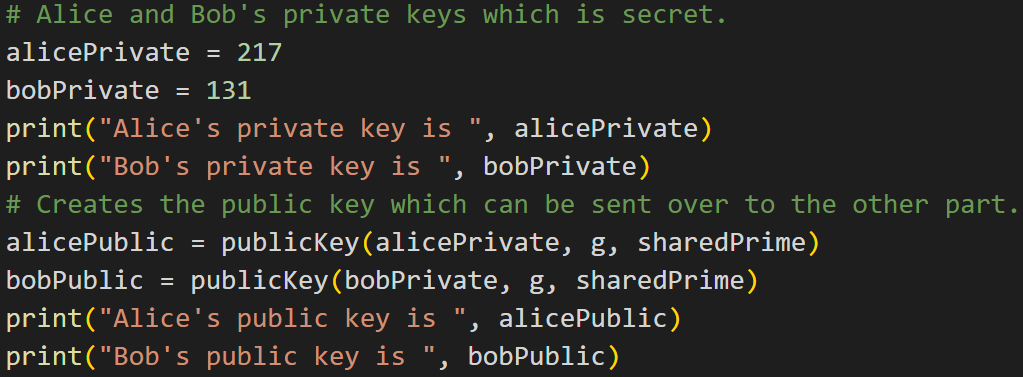
\includegraphics[width=\linewidth]{code_snippets/step2.PNG}
  \caption{Defines private key and calls a function to create the public key}
  \label{fig:step2}
\end{figure}

The third step is to send the public key to the part you want to connect with. Since this is a staged scenario and both Alice and Bob runs on the same program this is not necessary. But we will take a closer look into this step in part 2. 

The fourth step is to create a shared key. The shared key is created as shown in Figure \ref{fig:step4_func} by doing this operation: $$publickey^{privateKey} \ mod \ sharedPrime$$

\begin{figure}[H]
  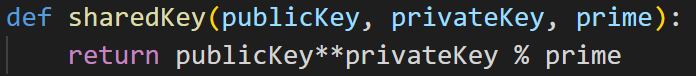
\includegraphics[width=\linewidth]{code_snippets/step4_func.PNG}
  \caption{The function to create the shared secret key}
  \label{fig:step4_func}
\end{figure}

Both Alice and Bob should now have the same shared key, which is a secret and should not be shared with anyone else. As shown in Figure \ref{fig:step4}, I check that the shared keys are the same for both Alice and Bob. If they do not have the same number something wrong happened along the way and they do not have a connection.

\begin{figure}[H]
  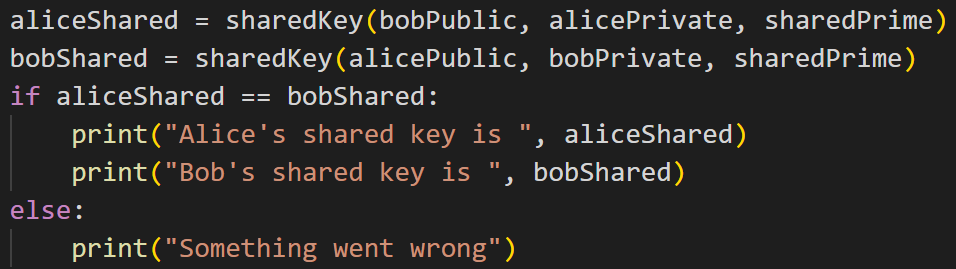
\includegraphics[width=\linewidth]{code_snippets/step4.PNG}
  \caption{Calls the function to get the shared key, and check if Alice and Bob have the same key}
  \label{fig:step4}
\end{figure}

At this point, we are done with the Diffie-Hellman's key exchange, but since Alice and Bob are concerned about the strength of the shared key, they want to use a cryptographically strong pseudo-random number generator (CSPRNG). I choose to use pseudo-random number generator named Blum Blum Shub (BBS) in this fifth step. Blum Blum Shub takes the form: $$x_{n+1} = x^{2}_{n} \ mod \ M$$
$x_{0}$ is called the seed, which in this case is the shared secret key. M is p*q where both q and p is a prime number and both are congruent to 3 mod 4. Both 7 and 11 fulfills that, and therefore I chose my M to be 7*11 = 77. This method is based on taking the least significant bit for each operation, as shown in Figure \ref{fig:step5}. On the way we have to check that the seed we start with or the new seeds that we creates not are 0 or 1. We do also have to check that the seed values not share factors with either p or q, Ref \cite{BBS}.

\begin{figure}[H]
  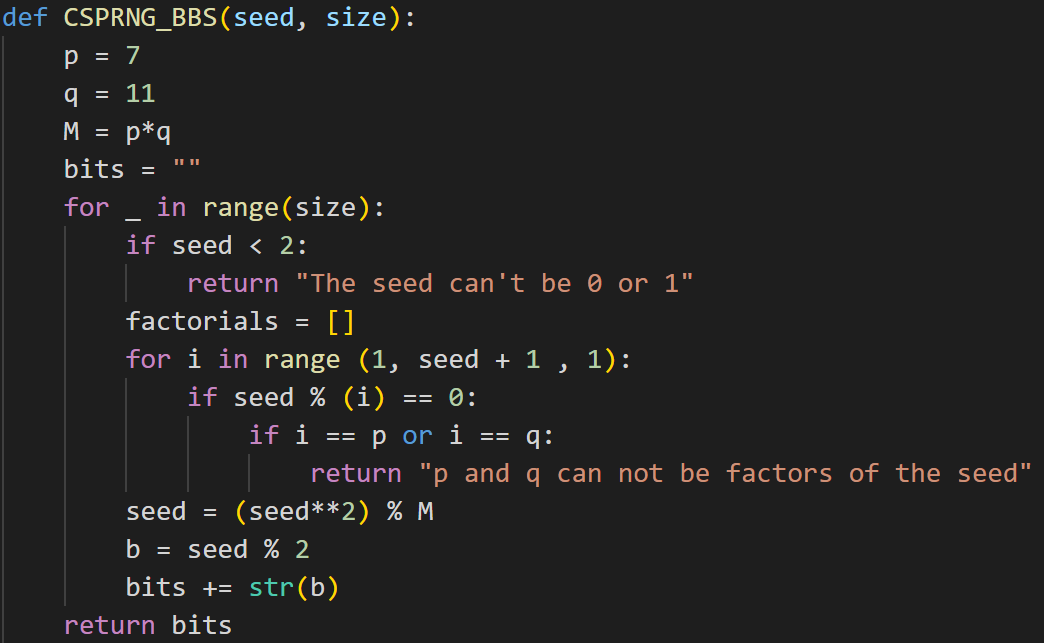
\includegraphics[width=\linewidth]{code_snippets/step5.PNG}
  \caption{The function that performs Blum Blum Shub}
  \label{fig:step5}
\end{figure}

As shown in Figure \ref{fig:step6} we uses the CSPRNG and creates a secret key which is of length 10 bits, but I convert it into a decimal. The reason why I chose a bit length of 10 is because In the next step we are going to encrypt a text and send it to Bob. For the encryption I chose to use SDES from the previous assignment. This is not a secure encryption, but since encryption is not the focus in this assignment I used SDES instead of importing something more secure. SDES encryption takes in a 10 bit long key and encrypts 8 bit blocks at a time. As shown in Figure \ref{fig:step6} you get the choice of writing your own message or using a predefined message. I convert the message into bits and split it up in 8 bit blocks. Then the program goes through the list of 8 bit block and encrypt them using our 10 bit key.

\begin{figure}[H]
  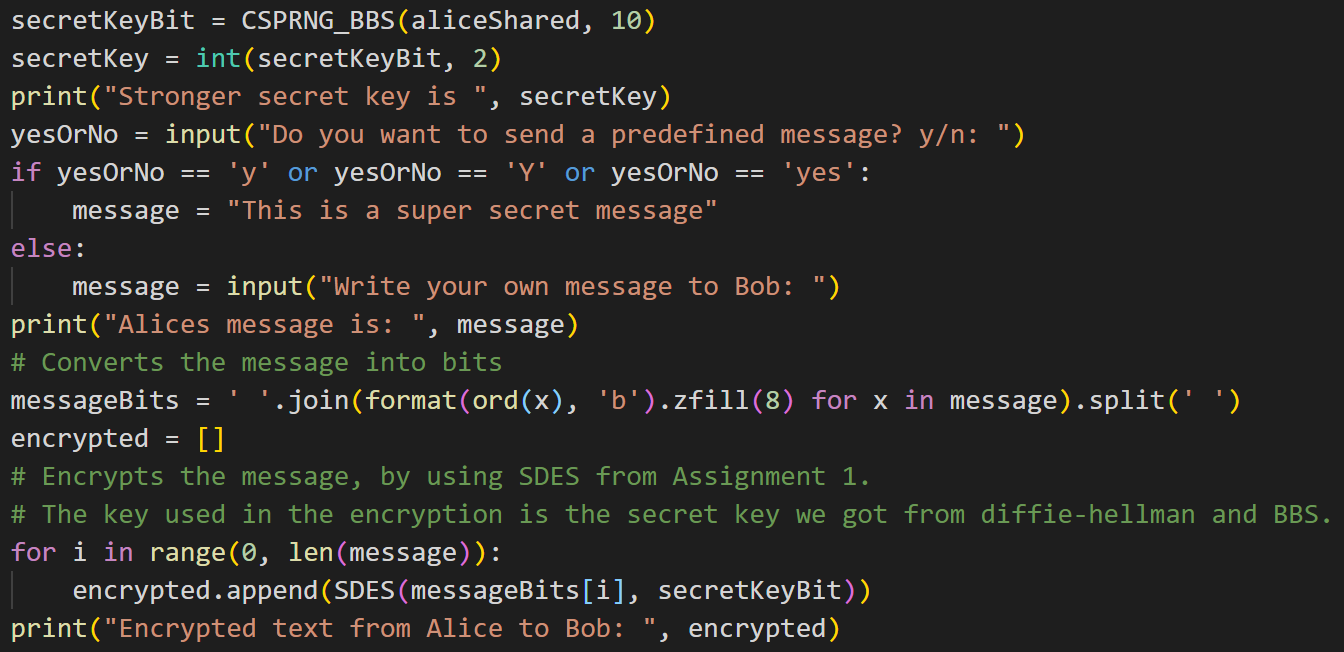
\includegraphics[width=\linewidth]{code_snippets/step6.PNG}
  \caption{Calls Blum Blum Shub and SDES to secure the key and encrypt a text}
  \label{fig:step6}
\end{figure}

The next step is for Bob to decrypt the message from Alice. At this point we already know that Alice and Bob got the same shared key and used the same BBS. So as shown in Figure \ref{fig:step7}, we take in 8 bit blocks from the cipher and decrypt it using the same key, which will give us the message from Alice in plaintext.

\begin{figure}[H]
  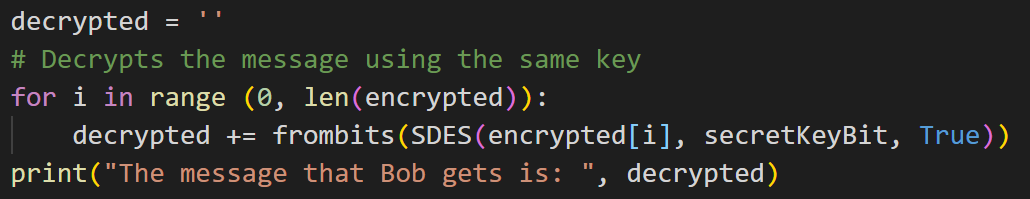
\includegraphics[width=\linewidth]{code_snippets/step7.PNG}
  \caption{Calles SDES to decrypt the cipher from Alice}
  \label{fig:step7}
\end{figure}

I have now shown a secure communication scenario between Alice and Bob. If someone else would have gotten the cipher, they could not have deciphered it, because the key was created from both Alice's private key and Bob's private key and their shared prime, which is a secret. 

\subsection*{Part 2}


\section*{Test results}
Results of testing the software, as you observed/recorded them. Note that this section is only for
observations you make during testing. Your analysis belongs in the Discussion section.

\section*{Discussion}
Your analysis of what your testing results mean, and your analysis.

\section*{Conclusion}
A short paragraph that restates the objective from your introduction and relates it to your results
and discussion, and describes any future improvements that you would recommend. Works Cited A
bibliography of all of the sources you got information from in your report.

\newpage
\begin{thebibliography}{10} 
\bibitem{BBS} A Security site,  \emph{Explaines how Blum Blum Shub works},
\url{https://www.asecuritysite.com/encryption/blum}.
\end{thebibliography}



\end{document}